\selectlanguage{ngerman}
\begin{ledgroupsized}[r]{120mm}
\footnotesize
\pstart
\noindent\textbf{Überlieferung:}
\pend
\end{ledgroupsized}
\begin{ledgroupsized}[r]{114mm}
\footnotesize
\pstart \parindent -6mm
\makebox[6mm][l]{\textit{L}}%
Konzept:
LH~XXXVII~3 Bl.~67.
Ein Blatt~4\textsuperscript{o};
alle Ränder beschnitten.
Zwei Seiten.
Der lange Zusatz auf \refpassage{37_03_067_1a}{37_03_067_1b} 
setzt am rechten Rand von Bl.~67~r\textsuperscript{o}, unmittelbar nach der auf \refnote{FnB:37_03_067_determinandum} ergänzten Frage, an und führt diese aus; er wurde, wie aus der Textverteilung ersichtlich ist, nachgetragen und nimmt die untere Hälfte von Bl.~67~r\textsuperscript{o} ein.
Eine weitere und spätere Textschicht auf Bl.~67~r\textsuperscript{o} bilden die Ausführungen über die Ursache der Festigkeit (\refpassage{37_03_067_4a}{37_03_067_4b}), die Leibniz im freigebliebenen Platz im oberen rechten Seitenbereich schrieb.
Auf Bl.~67~r\textsuperscript{o}, von Leibniz überschrieben, der eigh.\ Briefentwurf: 
\textit{Monsieur} \lbrack/\rbrack\ 
\textit{je serois faché de vous importuner sans sujet, mais} \lbrack/\rbrack\ 
\textit{voicy une raison, qui m'oblige de vous écrire.}
\pend
\end{ledgroupsized}
\vspace{5mm}
\begin{ledgroup}
\footnotesize
\pstart
\noindent%
\textbf{Datierungsgründe:}
Der Adressat des Briefentwurfs konnte bisher nicht identifiziert werden.
Wegen der Erwähnung von
\indexN{\textls{Huygens} (Hugenius, Ugenius, Hugens, Huguens), Christiaan 1629\textendash1695}Huygens' %
\cite{00525}\textit{Traité de la lumière}, Leiden 1690,
im Schlussteil des Konzepts (\refnote{FnC:37_03_067_Huygens})
bildet die erste Lektüre dieses Werkes, die, wie 
aus dem Briefwechsel mit \indexN{\textls{Mencke} (Menken, Menkenius, Menque), Otto 1644\textendash1707}O.~Mencke
(siehe \textit{LSB} III, 4 N. 281, bes. S.\;588) 
hervorgeht,
zwischen Mitte September und 12. Oktober 1690 stattgefunden haben muss, 
einen Terminus post quem für N.\;\ref{41780}.
Bereits ein kurzes Exzerpt aus dem \textit{Traité}, das bei dieser Lektüre entstanden sein muss (\cite{02094}\textit{LSB} VIII,~3 N.\;75), widmet sich derselben These über den Mehrkörperstoß, die  in N.\;\ref{41780} zum Thema wird.
\pend
\pstart			
Im langen Zusatz auf Bl.~67~v\textsuperscript{o} (\refpassage{37_03_067_1a}{37_03_067_1b})
erwähnt Leibniz die Methode der Stoßuntersuchung durch Dekomposition des Mehrkörpersystems in einfachere Teilsysteme, deren Kräfte separat berechnet und anschließend (als \textit{vires respectivae}) wieder zusammengesetzt werden können. Er nennt dies \glqq regula mea\grqq\ und veranschaulicht sie zudem durch das Modell des in einem Schiff bewegten zweiten Schiffs.
Allerdings scheint er zugleich diese Methode als weiterer Begründung und Bestätigung bedürftig anzusehen, im Gegensatz zu seinen Aussagen in den Konzepten N.\;\ref{58300} und N.\;\ref{58293}, in denen er sie für nunmehr ausgemacht und zuverlässig ansieht.
Diese Tatsache lässt die Vermutung zu, dass N.\;\ref{41780} vor den letzgenannten Stücken entstanden sei. Die Endpunkten ihrer erschlossenen Datierungsspannen (7. Februar 1696 für N.\;\ref{58300} und  1696 für N.\;\ref{58293}) ergeben auch für N.\;\ref{41780} den Terminus ante quem 1696.
\pend
\end{ledgroup}
\selectlanguage{latin}
\vspace{8mm}
\pstart%
\normalsize%
\noindent%
\edtext{\href{\Scan{LH_37_03_067r}}{\lbrack67~r\textsuperscript{o}\rbrack}
An ex solo principio conservandarum virium\indexS{principium conservandarum virium}\indexS{conservatio virium} omnia duci non possunt? Ex.~gr.}{%
\lemma{\href{\Scan{LH_37_03_067r}}{\lbrack67~r\textsuperscript{o}\rbrack}}%
\Bfootnote{%
\textit{(1)}~Ex solo \lbrack...\rbrack\ possunt, ex.~gr. %
\textit{(2)}~An ex \lbrack...\rbrack\  possunt? Ex.~gr.~\textit{L}}}
si globus\indexS{globus}\indexS{incursus globi in duo} \textit{A} incurrit in globos \textit{B}, \textit{C}, ex statu 1. fit status 2. Itaque
\edtext{accedit ut}{\lemma{accedit}\Bfootnote{%
\textit{(1)}~conservatio status prioris %
\textit{(2)}~ut~\textit{L}}} 
quam maxime obtineatur intentum.%
\pend
\vspace{1em}
\pstart
\begin{edtabularl}
\parbox{25mm}{%
\rule[-2mm]{0pt}{10mm}%
\protect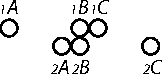
\includegraphics[scale=1]{gesamttex/edit_VIII-4/images/LH_37_03_067_d01a_067r.pdf}
\newline An sic potius \newline \rule{0pt}{16.3mm}%
\protect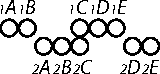
\includegraphics[scale=1]{gesamttex/edit_VIII-4/images/LH_37_03_067_d01b_067r.pdf}}
& 
\hspace{1.5em}%
\parbox{35mm}{%
\rule[-2mm]{0pt}{10mm}%
\protect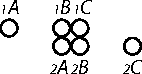
\includegraphics[scale=1]{gesamttex/edit_VIII-4/images/LH_37_03_067_d01c_067r.pdf}
\newline An sic \newline \rule{0pt}{16.3mm}%
\protect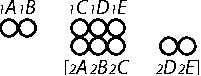
\includegraphics[scale=1]{gesamttex/edit_VIII-4/images/LH_37_03_067_d01d_067r.pdf}}
&
\parbox{40mm}{%
\rule[-2mm]{0pt}{16.3mm}
\newline Quid si \textit{DEF} cohaereant? \newline \rule{0pt}{16.3mm}%
\protect\raisebox{1.0ex}{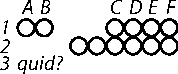
\includegraphics[scale=1]{gesamttex/edit_VIII-4/images/LH_37_03_067_d01e_067r.pdf}}}
\end{edtabularl}
\pend
\nopagebreak\vspace{0.5em}\startlock\nopagebreak
\pstart\centering
\edtext{\lbrack\textit{Fig.~1}\rbrack}{%
\lemma{\lbrack\textit{Fig.~1}\rbrack}%
\Cfootnote[nonum]{%
Im letzten Teildiagramm hat Leibniz die Punktbezeichnungen
\textit{\ind{1}A}, \dots\ \textit{\ind{1}E} doppelt vergeben.
Die dazugehörigen Indices ändert Hrsg.}}
\pend
\endlock
\vspace{1em}
\pstart
An efficitur, ut non solum centrum\indexS{centrum gravitatis omnium} omn.\ \textit{ABC} eadem celeritate procedat
\edtext{sed et \textit{A}}{\lemma{sed et}\Bfootnote{%
\textit{(1)}~centr. gr. %
\textit{(2)}~\textit{A}~\textit{L}}} 
et centr. gr.\indexS{centrum gravitatis} \textit{BC}, eadem celeritate a se invicem
\edtext{separentur; et \textit{C}}{\lemma{separentur; et}\Bfootnote{%
\textit{(1)}~\textit{A} et centr. gr %
\textit{(2)}~\textit{C}~\textit{L}}} 
et centr. gr.\indexS{centrum gravitatis} \textit{AB} similiter ut ante; an et \textit{B} et
\edlabel{37_03_067_2a}%
\edtext{}{%
\xxref%
{37_03_067_2a}{37_03_067_2b}%
\lemma{centr. gr. \textit{AC}.}\Bfootnote{%
\textit{(1)}~An pe %
\textit{(2)}~An~\textit{L}}}%
centr. gr. \textit{AC}.
\pend
\pstart
An%
\edlabel{37_03_067_2b}
cum inaequalia sunt corpora, et hoc perfecte
\edtext{obtineri semper}{\lemma{obtineri}\Bfootnote{%
\textit{(1)}~potest %
\textit{(2)}~semper~\textit{L}}}
non potest?
\edtext{Et an eo casu %
is motus erit, quo proxime accedetur, ut eo minor sit declinatio, a priori, quo major moles?
\edtext{Nempe determinandum qua ratione maxime accedatur ad priora.}{%
\lemma{}%
\applabel{FnB:37_03_067_determinandum}
\Bfootnote{Nempe \lbrack...\rbrack\ priora. \textit{erg.~L}}}%
}{\lemma{\textit{Am Rand}:}\Afootnote{NBNB}}
\pend 
\pstart 
An sufficit%
\edtext{}{\lemma{}\Afootnote{\textit{Am Rand}: Ita est}} 
\edtext{regula mea,\indexS{regula de summa virium respectivarum}}{%
\lemma{regula mea}%
\Cfootnote{Siehe bspw.
N.\;\ref{58300} und
N.\;\ref{58293} in diesem Band.}}
\edtext{ut summa ex vi}{%
\lemma{ut}%
\Bfootnote{%
\textit{(1)}~summa vis %
\textit{(2)}~summa ex vi~\textit{L}}} 
respectiva\indexS{vis respectiva}\indexS{summa virium respectivarum} 
inter \textit{A} et \textit{BC} juncta vi respectivae inter \textit{B} et 
\edtext{\textit{C}\lbrack;\rbrack\ item summa ex vi respectiva\indexS{vis respectiva} inter \textit{AB} et \textit{C} juncta}{%
\lemma{\textit{C}}%
\Bfootnote{%
\textit{(1)}~aequetur et vi respectivae inter \textit{AB} et \textit{C} junctae %
\textit{(2)}~item \lbrack...\rbrack\ juncta~\textit{L}}}
vi respectivae\indexS{vis respectiva} inter \textit{A} et \textit{B}; item summa ex vi respectiva\indexS{vis respectiva} inter \textit{AC} et \textit{B}, juncta vi respectivae\indexS{vis respectiva} inter \textit{A} et \textit{C}, semper conficiant idem, scil.\ vim respectivam\indexS{vis respectiva} priorem. 
Pro regulae hujus majore securitate videamus utrum ante concursum hic calculus virium respectivarum\indexS{vis respectiva} procedat.%
\edtext{}{\lemma{}\Afootnote{\textit{Hinter} procedat:\enskip NB. Video jam si succedit nihil determinare, quia ex uno sponte sequuntur et reliqua. An ergo adhibend. NB NB}}
\pend 
\pstart Vis ictus\indexS{vis ictus} inter duo est quadratum
\edtext{motus proprii,\indexS{motus proprius}}{\lemma{}\Bfootnote{motus \bars{motus \textit{streicht Hrsg.}} proprii,~\textit{L}}}
seu quo accedunt ad \indexS{centrum gravitatis commune}centrum commune grav.\lbrack,\rbrack\ 
ductum in molem.\indexS{moles}
\pend
\pstart
Vis ictus 
\edtext{inter tria\indexS{vis ictus inter tria}}{%
\lemma{}%
\Bfootnote{inter tria \textit{erg.~L}}} 
an itidem aestimari 
\edtext{potest quadratis celeritatum\indexS{quadratum celeritatis}}{%
\lemma{potest}%
\Bfootnote{%
\textit{(1)}~celeritate %
\textit{(2)}~quadratis celeritatum~\textit{L}}}
accedendi ad centr. com.,\indexS{centrum gravitatis commune} quod fingitur quiescere.
\edtext{Alius est sane modus inquirendi, si unum conferatur cum centro duorum,\indexS{centrum gravitatis duorum} et deinde reliqua inter se.}{%
\lemma{}%
\Bfootnote{Alius \lbrack...\rbrack\ se. \textit{erg.~L}}}
\pend
\begin{edfigure}			%
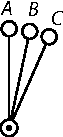
\includegraphics[scale=1]{gesamttex/edit_VIII-4/images/LH_37_03_067_d02_067r.pdf}
\edcaption{\lbrack\textit{Fig.~2}\rbrack}
\end{edfigure}
\pstart Si in circulum disposita sint \textit{A}, \textit{B}, \textit{C}, an ne idem eventus concursuum\indexS{concursus in circulo} ut in linea recta?
\pend
\vspace{0.5em}
\pstart
\noindent
\lbrack%
\textit{Der nachfolgende Zusatz bis \refpassage{37_03_067_1b}{37_03_067_1b} setzt unmittelbar nach der Ergänzung auf \refnote{FnB:37_03_067_determinandum} an:}\rbrack
\pend
\nobreak
\vspace{0.5em}
\pstart 
\noindent
\edlabel{37_03_067_1a}%
\edtext{Hic duo}{\lemma{Hic}\Bfootnote{%
\textit{(1)}~plura %
\textit{(2)}~duo~\textit{L}}} 
centra gravitatis partialia\indexS{centrum gravitatis partiale}
\edtext{quaevis}{\lemma{}\Bfootnote{quaevis \textit{erg.~L}}} 
eadem celeritate a se recedent
qua concurrerunt. Et an hoc sufficit ad determinandum? 
Nempe examinetur ante concursum,\indexS{concursus} an duo centra partialia\indexS{centrum gravitatis partiale}
eadem 
\edtext{celeritate sibi}{\lemma{celeritate}\Bfootnote{%
\textit{(1)}~concurrunt %
\textit{(2)}~sibi~\textit{L}}} 
accedunt, hoc video ita esse, quia nullo existente concursu, unumquodque uniformiter pergit.
Si haec succedunt\lbrack,\rbrack\ ut 
\edtext{arbitror, an consequens}{%
\lemma{arbitror,}%
\Bfootnote{%
\textit{(1)}~consequens %
\textit{(2)}~an consequens~\textit{L}}}
erit duo quaevis corpora eandem vim respectivam\indexS{vis respectiva} servare\indexS{conservatio vis respectivae} 
inter se, et tria quaevis
\edtext{itidem, et ita porro.}{\lemma{itidem,}\Bfootnote{%
\textit{(1)}~. Nam si sint  %
\textit{(2)}~et ita porro.~\textit{L}}} 
Nam si sint tria corpora \textit{A}, \textit{B}, \textit{C}, si \textit{A} et centr. \textit{BC} eadem qua ante celeritate a se invicem recedunt,
\edtext{erit ea pars}{\lemma{erit}\Bfootnote{%
\textit{(1)}~hactenus %
\textit{(2)}~ea pars~\textit{L}}} 
vis respectivae\indexS{vis respectiva} eadem quae
\edtext{ante. Sed}{\lemma{ante.}\Bfootnote{%
\textit{(1)}~Sed %
\textit{(2)}~Sed~\textit{L}}} 
cum tota sit eadem quae ante, etiam residua eadem erit, quae
\edtext{ante. Residua}{\lemma{ante.}\Bfootnote{%
\textit{(1)}~Ante aut %
\textit{(2)}~Residua~\textit{L}}} 
\edtext{a.}{%
\lemma{a.}%
\Cfootnote{%
\textit{autem}}}
tam ante quam post concursum est ipsa partialis vis respectiva\indexS{vis respectiva partialis} inter \textit{B} et \textit{C}. 
Videtur etiam forte hoc ex eo sequi, quia alioqui definiri poteret, in quo sit motus; quod examinandum.
\edtext{Imo falsam esse video consequentiam,}{\lemma{Imo}\Bfootnote{%
\textit{(1)}~hoc falsum esse video, \bars{et \textit{streicht Hrsg.}}
\textit{(a)}~institui perc
\textit{(b)}~poterit enim
\textit{(2)}~falsam esse video consequentiam,~\textit{L}}} 
quia duo corpora concurrentia sola sive constantia ex partibus unitis sive dissolutis eandem servant inter se vim respectivam,\indexS{conservatio vis respectivae} etiam
\edtext{du\lbrack o\rbrack}{\lemma{}\Bfootnote{duae \textit{L ändert Hrsg.}}} 
quaevis partialia\indexS{centrum gravitatis partiale} servare
\edtext{\lbrack debent\rbrack.}{%
\lemma{}%
\Bfootnote{debent \textit{erg.~Hrsg.}}}
\pend
\pstart
\edtext{Videndum an ex hypothesi respectivi motus\indexS{hypothesis motus respectivi}}{\lemma{Videndum}\Bfootnote{%
\textit{(1)}~quid %
\textit{(2)}~an ex
\textit{(a)}~casu %
\textit{(b)}~hypothesi %
\textit{(aa)}~motus %
\textit{(bb)}~respectivi motus~\textit{L}}}
seu indiscernibilis hypotheseos\indexS{hypothesis indiscernibilis} sequatur
\edtext{solutio. Finge}{\lemma{solutio.}\Bfootnote{%
\textit{(1)}~Fingo %
\textit{(2)}~Finge~\textit{L}}} 
duo \textit{B} et \textit{C} esse in navi\indexS{navis} mota motu eorum centri gr.\indexS{centrum gravitatis} 
Et hanc 
\edtext{navim in navi majore\indexS{navis in navi}}{%
\lemma{navim in navi}%
\Bfootnote{%
\textit{(1)}~mota %
\textit{(2)}~majore mota~\textit{L}}}
centr. gr. com. omnium\indexS{centrum gravitatis commune omnium} et \textit{A} moveri in hac navi majori. 
Quod si navis\indexS{navis} minor et \textit{A} non eadem celeritate qua venere a se invicem recedunt, 
sed diversis pro diversis celeritatibus, poterit discerni quantum motus sit in \textit{B}, 
et quantum in navi\indexS{navis} minori, etc.
Oportet ut celeritas recedendi\indexS{celeritas recedendi} sit qua venere. \pend
\pstart 
Adde hoc, nisi celeritas maneret eadem non reproducerentur priora
\edtext{licet pro re nata}{\lemma{licet}\Bfootnote{%
\textit{(1)}~re nata %
\textit{(2)}~res n %
\textit{(3)}~pro re nata~\textit{L}}} 
eo iretur. 
\pend
\pstart 
Idem etiam probatur ex natura actionis et reactionis aequalis,\indexS{actio et reactio aequales} poni enim potest \textit{A} agere in \textit{BC}, 
et haec reagere, adeoque eundem
\edtext{esse conatum}{\lemma{esse}\Bfootnote{%
\textit{(1)}~conatum reagendi %
\textit{(2)}~conatum~\textit{L}}}
a se discedendi.\indexS{conatus discedendi}
\pend
\begin{edfigure}%
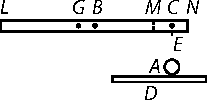
\includegraphics[scale=1]{gesamttex/edit_VIII-4/images/LH_37_03_067_d03_067r.pdf}
\edcaption{\edtext{\lbrack\textit{Fig.~3}\rbrack}{%
\lemma{\lbrack\textit{Fig.~3}\rbrack}%
\Cfootnote[nonum]{%
Ein gestrichener Entwurf zum Diagramm wird nicht wiedergegeben.}}}
\end{edfigure}
\pstart 
\edtext{Cum corpora concurrant eccentrice\indexS{concursus eccentricus} ut \textit{A} et
\edtext{\textit{B}, eodem modo videtur}{\lemma{\textit{B},}\Bfootnote{%
\textit{(1)}~et se
\textit{(2)}~eodem modo
\textit{(a)}~pergit %
\textit{(b)}~videtur~\textit{L}}} 
fieri ictus, ac si concurrerent tantum \textit{A} et \textit{C}.%
}{\lemma{}\Afootnote{\textit{Zwischen den Zeilen, oberhalb} eodem \lbrack...\rbrack\ concurrerent:\enskip Imo non puto, totum in motum concitandum\lbrack,\rbrack\ licet is gyrationis\indexS{motus gyrationis}}}
Datur ergo regressus\indexS{regressus} ipsius \textit{A}\lbrack,\rbrack\ datur et progressus centri gravitatis\indexS{progressus centri gravitatis} \textit{A} et \textit{B}, hinc dabitur et
\edtext{situs ipsius}{\lemma{}\Bfootnote{situs \bars{situs \textit{streicht Hrsg.}} ipsius~\textit{L}}} 
\textit{B}. Et quia datur vis respectiva inter \textit{A} et \textit{B} ex elongatione,\indexS{elongatio} 
oportet, ut quod deest vi respectivae\indexS{vis respectiva} priori, 
quaeratur in circulatione\indexS{circulatio} ipsius corporis oblongi\indexS{corpus oblongum} 
circa suum centrum\indexS{centrum gravitatis} \textit{B}; si duo oblonga\indexS{corpus oblongum} 
\edtext{concurrant, ut \textit{B} et \textit{D} res}{\lemma{concurrant,}\Bfootnote{%
\textit{(1)}~res mi %
\textit{(2)}~ut \textit{B} et \textit{D} res~\textit{L}}} 
minus faciles habet explicatus.
Videtur tamen ictus semper a centraliter obstante parte esse sumendus, deinde res concipienda, ac si
\edtext{pars illa}{\lemma{pars}\Bfootnote{%
\textit{(1)}~illa a re %
\textit{(2)}~illa~\textit{L}}} 
jam in motu posita ex
\edtext{legibus ante}{\lemma{legibus}\Bfootnote{%
\textit{(1)}~alibi %
\textit{(2)}~ante~\textit{L}}} 
determinatis a parte reliqua caperetur. 
Et quae est vis earum respectiva ante momentum rupturae\lbrack,\rbrack\ ea est vis
\edtext{circulationis.\indexS{vis circulationis} Vis}{\lemma{circulationis.}\Bfootnote{%
\textit{(1)}~Vis sc. respectiva inter ipsas part %
\textit{(2)}~Vis~\textit{L}}} 
sc. circulationis, est vis respectiva\indexS{vis respectiva} inter partes
\textit{LM}, et \textit{MN}, redactas in sua centra \textit{C} et \textit{G} circulantes circa commune centrum\indexS{centrum gravitatis commune} \textit{B}, haec enim
\edtext{si liberantur}{\lemma{si}\Bfootnote{%
\textit{(1)}~liberari possunt %
\textit{(2)}~liberantur~\textit{L}}} 
invicem recedent, licet oblique.
\pend
\pstart
Finge motum ipsius \textit{B} (in eccentrico concursu)\indexS{concursus eccentricus} esse progressus, 
et praeterea ex ictu fieri circulationem\indexS{circulatio} circa \textit{B}, et in momento ictus liberari \textit{BN}, 
feretur duplici motu uno recto\indexS{motus rectus} ipsius \textit{B}, 
altero ex circulatione\indexS{circulatio} in rectum averso,\indexS{motus in rectum aversus} per tangentem. 
Fingamus praeterea \textit{BL} similiter liberatum pergere in contrariam partem, 
sed ibi aequali occurrere, a quo reflectatur motu quo venerat.
Res redibit
\edtext{ad viam sine}{%
\lemma{ad}%
\Bfootnote{%
\textit{(1)}~vias %
\textit{(2)}~viam sine~\textit{L}}}
circulatione.\indexS{circulatio}
\edtext{Unde determinari puto poterit q. fuerit circulatio.\indexS{circulatio}%
}{\lemma{}\Afootnote{\textit{Unterhalb} Unde \lbrack...\rbrack\ circulatio:\enskip \textls{Hoc puto optimum}.}}
\pend
\pstart 
Videndum an ex hoc quod eadem vis absoluta\indexS{vis absoluta} manet, et quod centr. gr. commune\indexS{centrum gravitatis commune} aequabiliter procedit, 
et quod post momentum ictus duo concurrentia, \textit{A} scil. et punctum \textit{E} eadem celeritate a se invicem recedunt qua
\edtext{concurrere, eccentricus}{\lemma{concurrere,}\Bfootnote{%
\textit{(1)}~res %
\textit{(2)}~eccentricus~\textit{L}}} 
concursus\indexS{concursus eccentricus} possit definiri. %
Nam dum \textit{E}, uti 
\textit{C}, circulare incipit circa \textit{B}
et dum totum \textit{CN} procedere incipit\lbrack,\rbrack\
hi duo motus simul sumti componunt totam celeritatem recessus\indexS{celeritas recessus} \textit{C} ab \textit{A}.%
\edlabel{37_03_067_1b}
\pend 
\begin{edfigure}%
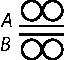
\includegraphics[scale=1]{gesamttex/edit_VIII-4/images/LH_37_03_067_d04_067r.pdf}
\edcaption{\lbrack\textit{Fig.~4}\rbrack}
\end{edfigure}
\pstart  
\edlabel{37_03_067_4a}%
Firmitatem corporum\indexS{firmitas corporum} venire necesse est a materia tenuissima,\indexS{materia tenuissima} 
cujus respectu solida nostra cribrorum\indexS{cribrum} instar habeant; quae 
corpora crassa\indexS{corpus crassum} a se invicem recedentia nonnihil, 
ob impulsus forte receptos, rursus ad se invicem pellat. 
\edtext{Alioqui ponenda}{%
\lemma{Alioqui}%
\Bfootnote{%
\textit{(1)}~ponendos %
\textit{(2)}~ponenda~\textit{L}}}
esset tractio,\indexS{tractio} non sola
\edtext{pulsio\indexS{pulsio}\lbrack,\rbrack\ dum}{\lemma{pulsio}\Bfootnote{%
\textit{(1)}~. Hujus actio %
\textit{(2)}~dum~\textit{L}}} 
intra brevissimum tempus in \textit{A} et \textit{B} innumeri ictus\indexS{ictus} ab aversis
\edtext{lateribus inferuntur}{\lemma{lateribus}\Bfootnote{%
\textit{(1)}~impingunt %
\textit{(2)}~inferuntur~\textit{L}}} 
qui has partes ad se invicem cogunt. Hinc
\edtext{si isti globuli\indexS{globulus}}{\lemma{si}\Bfootnote{%
\textit{(1)}~ista corpora %
\textit{(2)}~\bars{si \textit{streicht Hrsg.}} isti globuli~\textit{L}}} 
magneticis\indexS{globulus magneticus} similes adderentur, cum suis ictibus, 
utique appareret omnes motus esse rectilineos\indexS{motus rectilineus} in se, 
et per accidens ut curvilineos\indexS{motus curvilineus} considerari\lbrack,\rbrack\
neque adeo ob
\edtext{rece\lbrack de\rbrack ndi}{\lemma{}\Bfootnote{recededendi \textit{L ändert Hrsg.}}} 
a centro conatum\indexS{conatum recedendi a centrum} quicquam mutari 
de hypothesium aequivalentia.\indexS{aequivalentia hypothesium}
Accedit enim vis centripeta\indexS{vis centripeta} a 
\edtext{\lbrack curvi\rbrack lineo}{\lemma{}\Bfootnote{rectilineo \textit{L ändert Hrsg.}}}
motu.\indexS{motus rectilineus}\edlabel{37_03_067_4b}
\pend 
\pstart
\noindent
\href{\Scan{LH_37_03_067v}}%
{\lbrack67~v\textsuperscript{o}\rbrack}
\pend
\nobreak\begin{edfigure}[0.25em]%
\includegraphics[scale=1]{%
gesamttex/edit_VIII-4/images/LH_37_03_067_d05_067v.pdf}
\edcaption[0.25em]{\lbrack\textit{Fig.~5}\rbrack}
\end{edfigure}
\pstart
Conatus \textit{AC}, \textit{BC}, concurrunt in \textit{C} centro circuli.
Quod si id non sit centrum gravitatis\indexS{centrum gravitatis} sed aliud \textit{G}, sit tamen \textit{C} in directione ipsius \textit{G}, 
perinde est
ac si centrum gr.\indexS{centrum gravitatis} quoque esset
\edlabel{37_03_067_3a}%
\edtext{}{%
\xxref%
{37_03_067_3a}{37_03_067_3b}%
\lemma{in}%
\Bfootnote{%
\bars{\textit{G} \textit{ändert Hrsg.}}
\textit{(1)}~\bars{Si \textit{streicht Hrsg.}} di %
\textit{(2)}~Sit baculus \textit{BCG}, %
\textit{(a)}~in cujus %
\textit{(b)}~et~\textit{L}}}%
in \lbrack\textit{C}\rbrack.
\pend
\begin{edfigure}[0.5em]%
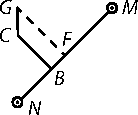
\includegraphics[scale=1]{gesamttex/edit_VIII-4/images/LH_37_03_067_d06_067v.pdf}
\edcaption{\lbrack\textit{Fig.~6}\rbrack}
\end{edfigure}
\pstart
Sit baculus \textit{BCG}, et%
\edlabel{37_03_067_3b}
sit impulsus in \textit{BC}, grave autem sit in altero extremo \textit{G}. 
An idem est, ac si impulsus fieret in \textit{FG} parallela ipsi \textit{BC}. %
\pend
\pstart
Sed hinc porro sequitur, si motus ille directus\indexS{motus directus} 
in linea \textit{BC} oriatur ex circulari\indexS{motus circularis} circa centrum \textit{M}, 
interesse, utrum grave sit in \textit{C} an vero in \textit{G} quia \textit{C} vecti\indexS{vectis} \textit{MFB} 
incumbet in \textit{B}, at \textit{G} in \textit{F}, propius ad centrum. Hinc etsi \textit{MB} 
et \textit{NB} sint aequales si tamen centrum grav.\indexS{centrum gravitatis} sit in \textit{G}, multum interest, 
utrum centrum motus sit \textit{N}, an \textit{M}, quia \textit{F} magis ab \textit{N} abest quam ab \textit{M}. 
Hoc prima fronte non apparebat. 
Et hinc video non posse tuto motus circulares\indexS{motus circularis} pro conatibus rectilineis\indexS{conatus rectilineus} substitui, etsi circulares quoque sint rectilinei in tangente.
\pend 
\begin{edfigure}[0.25em]%
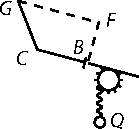
\includegraphics[scale=1]{gesamttex/edit_VIII-4/images/LH_37_03_067_d07_067v.pdf}
\edcaption{\lbrack\textit{Fig.~7}\rbrack}
\end{edfigure}
\pstart Si ope baculi
\edtext{curvi}{\lemma{}\Bfootnote{curvi \textit{erg.~L}}} 
\textit{BCG}, grave \textit{G} impellatur linea \textit{BC} vi ponderis \textit{Q}, perinde est quasi impulsus factus fuisset linea \textit{FG}, quia in hac
\edtext{linea ipsum}{\lemma{linea }\Bfootnote{%
\textit{(1)}~\textit{G} tendit %
\textit{(2)}~ipsum~\textit{L}}}
grave\indexS{grave} \textit{G} tendit.
\pend
\begin{edfigure}[2em][1em]    	%
\includegraphics[scale=1]{%
gesamttex/edit_VIII-4/images/LH_37_03_067_d08_067v.pdf}
\edcaption[0.25em]{\lbrack\textit{Fig.~8}\rbrack}
\end{edfigure}
\pstart Si \textit{A} incurrat in \textit{B} et \textit{C}, ita tamen ut tantum tangat \textit{B}, quid fiet? \pend 
\pstart Summa virium\indexS{summa virium} data est $Avv+Bee+%
\edtext{C\lbrack rr\rbrack$.}{%
\lemma{}%
\Bfootnote{\textit{Cr} \textit{L ändert Hrsg.}}}%
\pend
\pstart\noindent
$(A)((A))=v$. $(B)((B))=e$. $(C)((C))=r$. %
\pend
\pstart
Celeritas\indexS{celeritas centri gravitatis} et directio\indexS{directio centri gravitatis}
centr.\ grav.\ communis\indexS{centrum gravitatis commune} manet, 
seu quadratum ejus\indexS{quadratum celeritatis} ductum in Aggregatum.\indexS{quadratum celeritatis ductum in Aggregatum}
\pend
\pstart
Manere etiam debet eadem vis respectiva.\indexS{vis respectiva}
\pend
\pstart
Si ope horum determinari res
\edtext{potest, eadem}{\lemma{potest}\Bfootnote{%
\textit{(1)}~ut arbitror, determinabitur etiam, si fingamus %
\textit{(2)}~eadem~\textit{L}}} 
prodibunt, quae prodirent, si ponamus esse intervallum inter \textit{B} et \textit{C}, sed utcunque
\edtext{exiguum. Sed}{\lemma{exiguum.}\Bfootnote{%
\textit{(1)}~Nam %
\textit{(2)}~Sed~\textit{L}}} 
ea ratione semper quiescet \textit{A} post ictum si \textit{B} et \textit{C} 
\edtext{non cohaereant, sed}{%
\lemma{non cohaereant}%
\Bfootnote{%
\textit{(1)}~. Est %
\textit{(2)}~, sed~\textit{L}}}
quid si cohaereant? Tunc omnis vis respectiva\indexS{vis respectiva} redibit ad solum 
conatum discedendi\indexS{conatum discedendi} centri \textit{BC}
ab \textit{A}. Ergo haec duo confundi non debent. 
Sed si non cohaereant pars vis respectivae\indexS{vis respectiva} redacta erit ad recessum
inter \textit{B} et \textit{C}.
\pend 
\begin{edfigure}[1em][1em]    	%
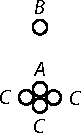
\includegraphics[scale=1]{gesamttex/edit_VIII-4/images/LH_37_03_067_d09_067v.pdf}\hspace*{20mm}
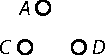
\includegraphics[scale=1]{gesamttex/edit_VIII-4/images/LH_37_03_067_d10_067v.pdf}
\edcaption[0.25em]{%
\edtext{\lbrack\textit{Fig.~9}\rbrack}{%
\lemma{\lbrack\textit{Fig.~9}\rbrack}%
\Cfootnote[nonum]{%
Ein gestrichener Entwurf zum Diagramm wird nicht wiedergegeben.}}%
\hspace*{22.5mm}
\lbrack\textit{Fig.~10}\rbrack\hspace*{2.5mm}}
\end{edfigure}
\pstart 
\edlabel{37_03_067_5a}%
Si globus\indexS{globus} \textit{A} simul tangat globos aequales plures\indexS{globus plures globos tangens} \textit{C}. 
et feriatur a globo \textit{B}, post ictum quiescent \textit{B} et \textit{A}, 
motusque omnis erit translatus\indexS{translatio omnis motus} in globos \textit{C}. 
\edtext{Hug.\ c.~1.\ \textit{Lum}.}{%
\applabel{FnC:37_03_067_Huygens}%
\lemma{Hug.\ c.~1.\ \textit{Lum}.}\Cfootnote{%
\indexN{\textls{Huygens} (Hugenius, Ugenius, Hugens, Huguens), Christiaan 1629\textendash1695}\textsc{C.~Huygens}, 
\textit{Traité de la lumière}, Leiden 1690\cite{00525}, 
chap.~1, S.\;14 mit Fig.\ (\textit{HO}\cite{00113} XIX, S.\;459\textendash477, hier S.\;473 mit Fig.~177). 
Siehe Leibnizens Auszüge aus dem einschlägigen Abschnitt des \cite{00525}\textit{Traité}:
\cite{02094}\textit{LSB} VIII,~3 N.\;75 von September\textendash Oktober 1690.%
}}
Ergo puto idem esse si \textit{A} incurrat in \textit{C} \textit{C} \textit{C} aequales,\indexS{incursus globi in plures aequales} 
sumamus duos tantum et consideremus quid futurum. Debet eadem
\edtext{esse vis\indexS{vis}}{\lemma{esse}\Bfootnote{%
\textit{(1)}~celeritas in sum %
\textit{(2)}~vis~\textit{L}}} 
in summa\lbrack,\rbrack\ a qua si detrahatur 
vis centri gravitatis\indexS{vis centri gravitatis} restabit vis ictus\indexS{vis ictus}\lbrack,\rbrack\
quem examinemus.
Videbimus et an idem prodeat, si paulo ante attingat \textit{C} quam \textit{D}.\edlabel{37_03_067_5b}%
\pend 
